% !TeX program = xelatex
\documentclass[UTF8,11pt,a4paper]{ctexart}

\usepackage[margin=24mm]{geometry}
\usepackage{graphicx}
\usepackage{amsmath}
\usepackage{booktabs}
\usepackage{longtable}
\usepackage{tabularx}
\usepackage{array}
\usepackage{float}
\usepackage{caption}
\usepackage{subcaption}
\usepackage{placeins}
\usepackage{xcolor}
\usepackage{enumitem}
\usepackage[hidelinks]{hyperref}

\graphicspath{{fig/}}
\setlength{\parindent}{2em}
\setlength{\parskip}{6pt}
\setlist[itemize]{leftmargin=*, topsep=2pt}
\setlist[enumerate]{leftmargin=*, topsep=2pt}

\newcommand{\mm}{\,\mathrm{mm}}
\newcommand{\Hz}{\,\mathrm{Hz}}
\newcommand{\pct}{\,\%}
\newcommand{\case}[1]{\texttt{#1}}
\newcommand{\tight}{\setlength{\tabcolsep}{4pt}\renewcommand{\arraystretch}{1.12}}

\title{\textbf{AutoPos UWB 场地实验评估报告}\\
\large 基于 OptiTrack 真值隔离的静态、动态、延迟耦合、滤波与鲁棒性分析}
\author{FULL Erlangen 2026-05-28 分析包}
\date{基于 corrected FULL 4-way comparison 与 reviewer-audit 输出生成，2026-06-04}

\begin{document}
\maketitle

\begin{abstract}
本文总结 Erlangen 2026-05-28 数据集上的 corrected FULL AutoPos/Vicon 分析。
报告把问题拆成 anchor layout 精度、layout-level residual delay 与布局坐标系耦合、
静态 tag 定位、ROTO 动态轨迹、post-solve 滤波、Pseudo-IMU oracle 融合以及鲁棒性诊断。
当前已经锁定的部署静态 headline 是：真实 production export path 切到 T4 tag solver 后，
仍保持 production mean aggregation，得到 original FULL \case{v4-io/T4}
\textbf{72.7 mm median / 171.5 mm P95 / 109.8 mm RMSE}。此前常见的
\textbf{69.7/173.9 mm} 是 median-estimator ablation，不再作为 deployed production
headline。动态 ROTO 在同一 \case{v4-io/T4} solver line 上仍为
\textbf{105.8 mm track-median P50 / 231.8 mm track-median P95}，说明动态绝对误差不会
仅靠静态 layout 或 delay control 直接塌缩。
新的 FULL-US 重跑对应 BioSpur AutoPos 的部署系统：UWB 加 US30/F-G-H 高度 gauge。
它并不会显著改变旧的 3D anchor-locked accuracy 数字；它真正解决的是 vertical gauge
与坐标系物理可解释性。按照新的 height-preserving evaluation，FULL-US \case{v4-io}
相对 OptiTrack 的静态 tag 结果为 \textbf{72.5 mm median / 284.8 mm P95 / 139.1 mm RMSE}。
\end{abstract}

\section{一页结论}

\begin{table}[H]
\centering
\tight
\caption{核心结果总表。静态 production 使用每个静态位置的 mean aggregation；
ROTO 使用 17 个旋转 capture、34 条 tag-track 的 track-median 汇总。}
\begin{tabularx}{\textwidth}{lXrrr}
\toprule
类别 & case & Median/P50 & P95 & RMSE 或关键诊断 \\
\midrule
静态部署 headline & FULL production mean-aggregated \case{v4-io/T4} & 72.7 & 171.5 & 109.8 RMSE \\
静态部署 gauge & FULL-US UWB+US30 height-preserving \case{v4-io} & 72.5 & 284.8 & 139.1 RMSE \\
Anchor 部署 gauge & FULL-US UWB+US30 height-preserving \case{v4-io} & 98.4 & 162.1 & 109.7 RMSE \\
静态 legacy production & FULL production mean-aggregated \case{v4-io/T1} & 74.0 & 282.1 & 139.6 RMSE \\
静态 estimator ablation & FULL median-estimator \case{v4-io/T4} & 69.7 & 173.9 & 108.9 RMSE \\
Known-anchor control & Vicon anchors + re-estimated delay, T4 & 64.1 & 128.4 & 77.7 RMSE \\
One-baseline control & E-H one-baseline + re-estimated delay, T4 & 58.1 & 130.2 & 78.4 RMSE \\
ROTO baseline & FULL original \case{v4-io/T4} & 105.8 & 231.8 & 141.3 sample RMSE \\
ROTO known-anchor control & Vicon anchors + re-estimated delay, T4 & 105.6 & 200.4 & 125.4 sample RMSE \\
ROTO fixed-lag filter & FULL original \case{T4+F4} & 86.3 & 158.2 & latency smoother 诊断 \\
ROTO pseudo-IMU oracle & FULL original \case{T4+PI1} & 66.1 & 97.5 & OptiTrack-derived motion prior \\
\bottomrule
\end{tabularx}
\end{table}

最重要的结论是：静态与动态是两类不同问题。静态 tag localization 对 layout/delay
处理和静态 dwell aggregation 很敏感；动态 ROTO 即使在 known-anchor + re-estimated-delay
control 下，绝对轨迹误差仍约为 10 cm median。因此动态残差不是一个简单的全局 scale
误差、不是一个常数 time offset 误差，也不是 0.8 ms protocol broadcast window 可以解释的误差。

\section{FULL-US：UWB + US30 高度 Gauge}

Original FULL 和 FULL-US 回答的是两个略有不同的问题。Original FULL \case{v4-io}
是 UWB AutoPos self-calibration，并使用历史上的 soft two-layer vertical prior。
FULL-US \case{v4-io} 则是在同一 AutoPos pipeline 上引入 US30/F-G-H ultrasound height gauge，
用它固定 vertical coordinate gauge。OptiTrack 仍然是外部 ground truth。

\begin{table}[H]
\centering
\tight
\caption{FULL、FULL-US 与 OptiTrack 的三方对比。除 reference 外，数值均为相对 OptiTrack 的 3D error，单位 mm。}
\begin{tabularx}{\textwidth}{lXrrr}
\toprule
系统 & 坐标含义 & Static tag P50/P95 & Anchor P50/RMSE & ROTO P50/P95 \\
\midrule
FULL \case{v4-io} & UWB AutoPos + soft two-layer Z prior；gauge 不是直接可部署的物理高度框架 & 74.0/282.1 legacy production & 92.8/105.4 & 105.8/231.8 \\
FULL-US \case{v4-io} & UWB AutoPos + US30/F-G-H height gauge；vertical gauge 具有部署物理意义 & 72.5/284.8 height-preserving & 98.4/109.7 height-preserving & 105.8/231.8 \\
OptiTrack & optical ground truth reference & reference & 0.28 mm coordinate-SD median & reference \\
\bottomrule
\end{tabularx}
\end{table}

最重要的结论是：FULL-US 不是一个让旧 accuracy 指标大幅提升的模块。在 no-US vs US 对比中，
10 个 legacy anchor-locked 行里有 8 个几乎完全不变，剩下两个 P95 变化也小于 0.12 mm。
这是预期现象，因为旧指标允许 full 3D anchor/capture alignment，它会把单纯的 coordinate-gauge
变化吃掉。

因此 US30 在论文里的贡献应这样写：它固定 BioSpur AutoPos 的 coordinate gauge，尤其是 vertical axis，
使输出坐标系在部署中具有物理可解释性；它本身并不会显著提高 UWB ranging accuracy。正确的部署诊断
是 height-preserving check：只允许水平 2D rigid transform 加一个 vertical shift，不允许任意 3D
pitch/roll 把 US height gauge 抹掉。在这个口径下，FULL-US \case{v4-io} 静态 tag 误差为
72.5/284.8 mm，RMSE 139.1 mm；anchor layout 误差为 98.4/162.1 mm，RMSE 109.7 mm。

\section{数据集、坐标框架与评估协议}

数据集来自 Erlangen 2026-05-28 corrected FULL OptiTrack export。主 infrastructure
配置为 AutoPos \case{v4-io}，并用 OptiTrack/Vicon anchor 与 tag truth 做验证。本文比较四条主路径：
\begin{itemize}
    \item original FULL self-calibrated AutoPos layout + solver residual corrections；
    \item Vicon/OptiTrack known anchor coordinates + 在该坐标框架上重新估计 residual delay；
    \item full Sim(3) scale-to-Vicon layout + 重新估计 residual delay；
    \item one-baseline E-H scale correction + 重新估计 residual delay。
\end{itemize}

静态结果来自 24 个固定 tag 位置。ROTO 结果来自 17 个 rotating capture，共 34 条 tag track。
静态 production 结果使用真实 production export path：每帧先解 tag 位置，再由
\case{position\_summary} 对每个静态位置做 mean aggregation。此次 production path 已经从 legacy T1
analytic solver 切到 T4 C-solver；mean aggregation 保持不变。真实 production T4 run 得到：
\[
72.691/171.493/109.843\mm
\]
probe 得到：
\[
72.689/171.497/109.845\mm
\]
二者在数值噪声内一致。因此 headline 采用 production mean-aggregated \case{v4-io/T4}
的 72.7/171.5/109.8 mm。

\section{指标定义}

\begin{itemize}
    \item \textbf{Static median/P95/RMSE：} 静态 tag 估计点与 corrected OptiTrack tag truth 之间的 3D error。
    \item \textbf{ROTO ATE：} solved UWB antenna samples 与插值后的 OptiTrack antenna marker 之间的 absolute trajectory error。
    \item \textbf{ROTO track-median：} 对每条 tag track 先算 summary，再取跨 track median，避免长 track 过度加权。
    \item \textbf{RPE：} frame-to-frame relative position error，用于评价局部运动一致性。
    \item \textbf{SE(3) layout error：} 对 anchor layout 做刚体/反射规范化对齐后的误差；它保留 global scale bias。
    \item \textbf{Sim(3) layout error：} 允许一个全局 scale factor 后的 similarity residual；它衡量去掉全局 scale 后的非均匀形变。
    \item \textbf{Residual delay correction：} 本文所有 \case{d\_anchor\_mm} 和 tag-delay 项都指 firmware antenna-delay setting
    16436 DTU 之上的 layout-level residual software correction。它们不能直接写成物理 antenna delay。
\end{itemize}

\section{Anchor Self-Positioning 精度}

\begin{figure}[H]
\centering
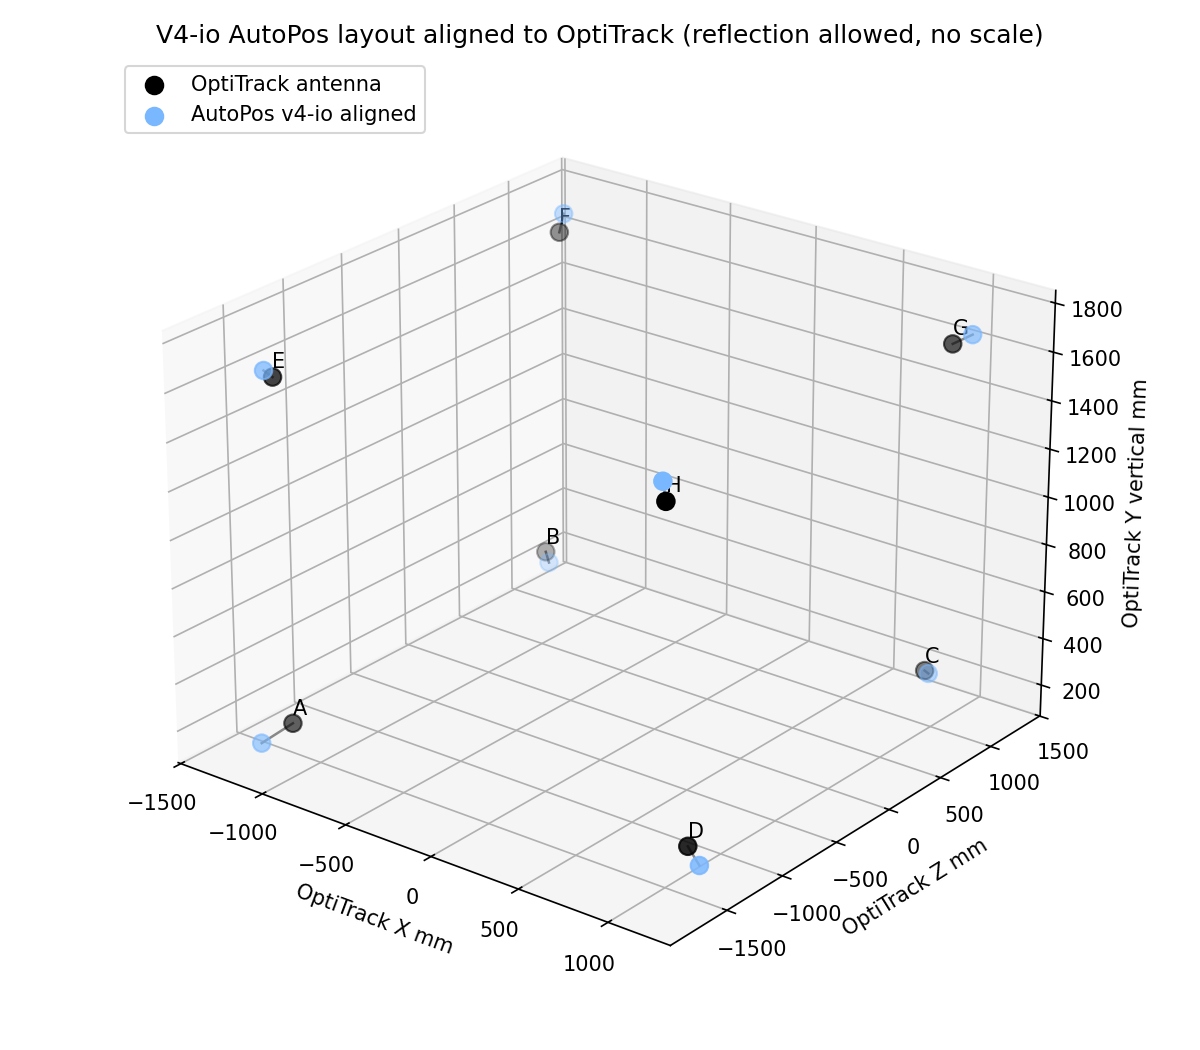
\includegraphics[width=0.88\textwidth]{layout_opti_vs_autopos_3d.png}
\caption{OptiTrack anchor layout 与 AutoPos layout 对比。关键不只是 3D anchor coordinate error，
还包括对齐后可以看到的 global scale shrinkage。}
\end{figure}

\begin{table}[H]
\centering
\tight
\caption{Anchor layout absolute accuracy。SE(3) 保留 scale bias；Sim(3) 去掉一个全局 scale 自由度。}
\begin{tabular}{lrrrrr}
\toprule
Method & SE(3) RMSE & Median & P95 & Scale bias & Sim(3) RMSE \\
\midrule
AutoPos v1-old & 101.3 & 84.6 & 154.1 & -4.50\% & 50.1 \\
AutoPos v4-io & 105.4 & 92.8 & 156.9 & -4.17\% & 67.1 \\
AutoPos v2 & 136.5 & 127.8 & 184.0 & -6.15\% & 60.3 \\
AutoPos v3-lite & 136.6 & 127.9 & 184.2 & -6.15\% & 60.9 \\
AutoPos v3-full & 143.4 & 118.9 & 211.7 & -3.61\% & 125.3 \\
\bottomrule
\end{tabular}
\end{table}

生产 layout \case{v4-io} 的 frame-normalized rigid SE(3) RMSE 为 105.4 mm，
Sim(3) residual 为 67.1 mm。Sim(3) scale 为 0.958267，说明 AutoPos layout 相比
OptiTrack layout 存在约 4.17\% 的全局收缩。Rigid RMS 与 similarity RMS 的差异不是计算 bug；
它反映的是 scale 这个额外自由度确实解释了部分 layout error。因此论文中 similarity RMS
应标记为 diagnostic，而不是部署场景下的 field accuracy headline。

\section{Delay-Layout Coupling}

\begin{figure}[H]
\centering
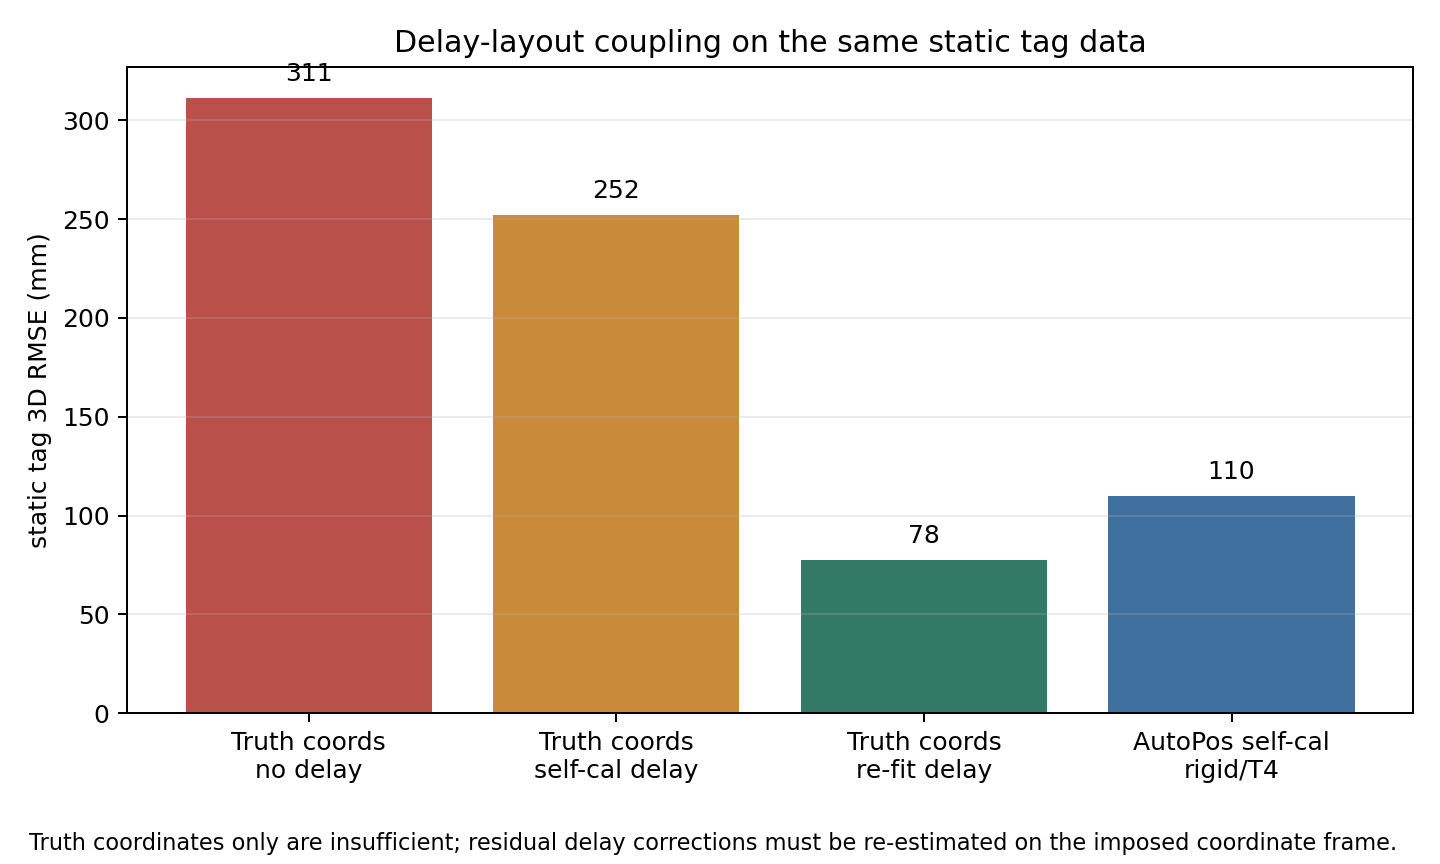
\includegraphics[width=0.78\textwidth]{delay_layout_coupling.png}
\caption{Delay-layout coupling triangle。仅施加 optical anchor coordinates 并不足够；
residual delay 必须在同一个 layout frame 上重新估计。}
\end{figure}

\begin{table}[H]
\centering
\tight
\caption{同一组静态 tag 数据在不同 layout 与 delay treatment 下的结果。}
\begin{tabularx}{\textwidth}{lXrr}
\toprule
Case & 解释 & RMSE & P95 \\
\midrule
Vicon truth, no delay correction & 只有 optical geometry 不够 & 311.3 & 453.4 \\
Vicon truth, transplanted self-cal delay & AutoPos residual corrections 不能直接移植 & 252.2 & 394.6 \\
Vicon truth, re-estimated delay & known-anchor + re-estimated-delay control & 77.7 & 128.4 \\
AutoPos v4-io, co-fitted delay & self-cal geometry 与 residual correction 共同条件化 & 108.9 & 174.1 \\
\bottomrule
\end{tabularx}
\end{table}

这是 OptiTrack-isolated 分析中最核心的机制结果。已知 anchor 坐标本身不能充分约束 tag solver；
endpoint residual delay model 必须在同一个 layout frame 上重新估计。这个机制也体现在 per-anchor
层面：WHY \#9 将 self-minus-Vicon \case{anchor\_main\_rel\_A} 对 \case{v4-io} radial layout error
做回归，得到 \(R^2=0.998\)、slope \(-0.982\mm/\mm\)。也就是说，self-cal residual delay term
几乎一比一吸收了 radial coordinate/scale error。这不是 solver sign bug，而是 gauge absorption。

\section{静态 Tag Positioning}

\begin{figure}[H]
\centering
\begin{subfigure}{0.49\textwidth}
\centering
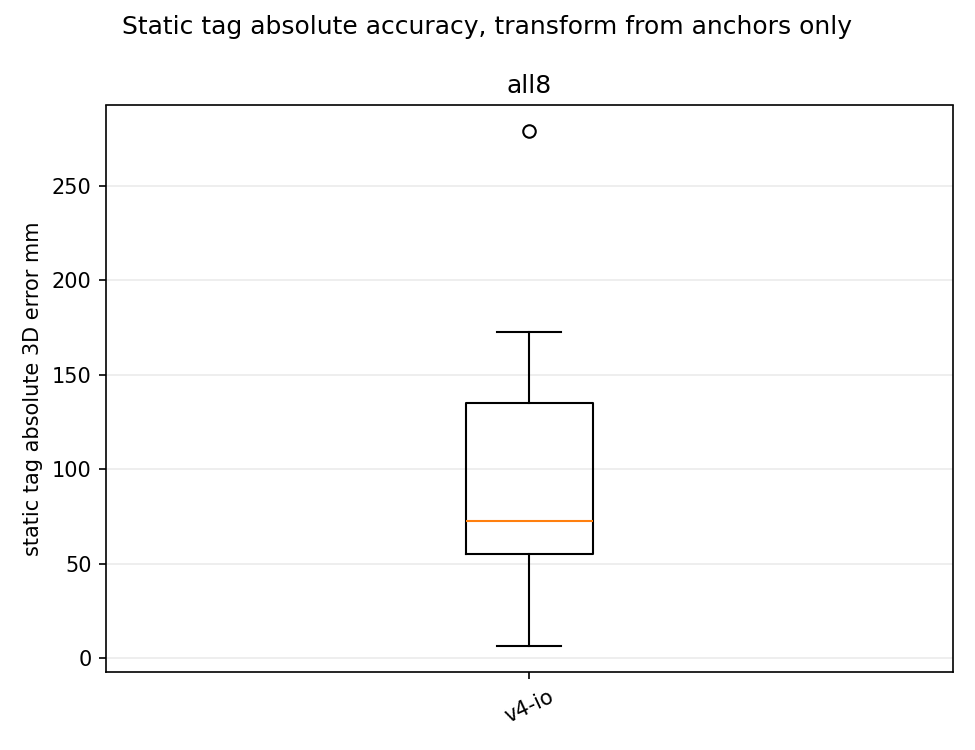
\includegraphics[width=\linewidth]{production_T4_tag_error_by_position.png}
\caption{Production T4 mean-aggregated static error by position。}
\end{subfigure}
\hfill
\begin{subfigure}{0.49\textwidth}
\centering
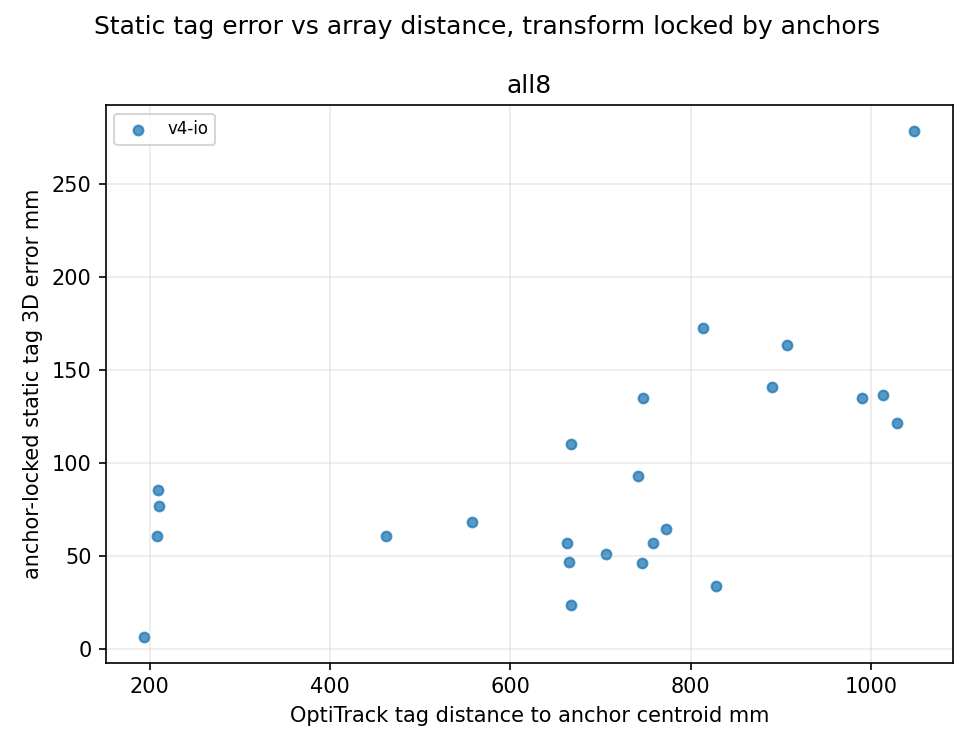
\includegraphics[width=\linewidth]{production_T4_tag_error_vs_distance.png}
\caption{Production T4 static error versus distance。}
\end{subfigure}
\caption{真实 production export path 切到 T4 后的静态结果；mean aggregation 保持不变。}
\end{figure}

\begin{table}[H]
\centering
\tight
\caption{静态 tag accuracy。}
\begin{tabularx}{\textwidth}{lXrrr}
\toprule
Case & 角色 & Median & P95 & RMSE \\
\midrule
Production mean \case{v4-io/T4} & deployed static headline & 72.7 & 171.5 & 109.8 \\
Legacy production mean \case{v4-io/T1} & old exported production path & 74.0 & 282.1 & 139.6 \\
Median-estimator \case{v4-io/T4} & estimator-sensitivity ablation & 69.7 & 173.9 & 108.9 \\
Median-estimator \case{v4-io/T3} & estimator-sensitivity ablation & 69.2 & 173.0 & 106.6 \\
Vicon truth + re-estimated delay & known-anchor control & 64.1 & 128.4 & 77.7 \\
Sim(3) scale + re-estimated delay & global scale removed & 67.1 & 132.6 & 81.6 \\
One-baseline E-H + re-estimated delay & field-measurable scale control & 58.1 & 130.2 & 78.4 \\
\bottomrule
\end{tabularx}
\end{table}

Production 与 replay 的口径必须分开。69.7/173.9 mm 不是 deployed static point；
它是 raw replay/evaluation path 中使用 median estimator 的 ablation。部署导出的 production static point
使用 mean aggregation；真实 production T4 结果是 72.7/171.5 mm，RMSE 109.8 mm。

\begin{figure}[H]
\centering
\begin{subfigure}{0.49\textwidth}
\centering
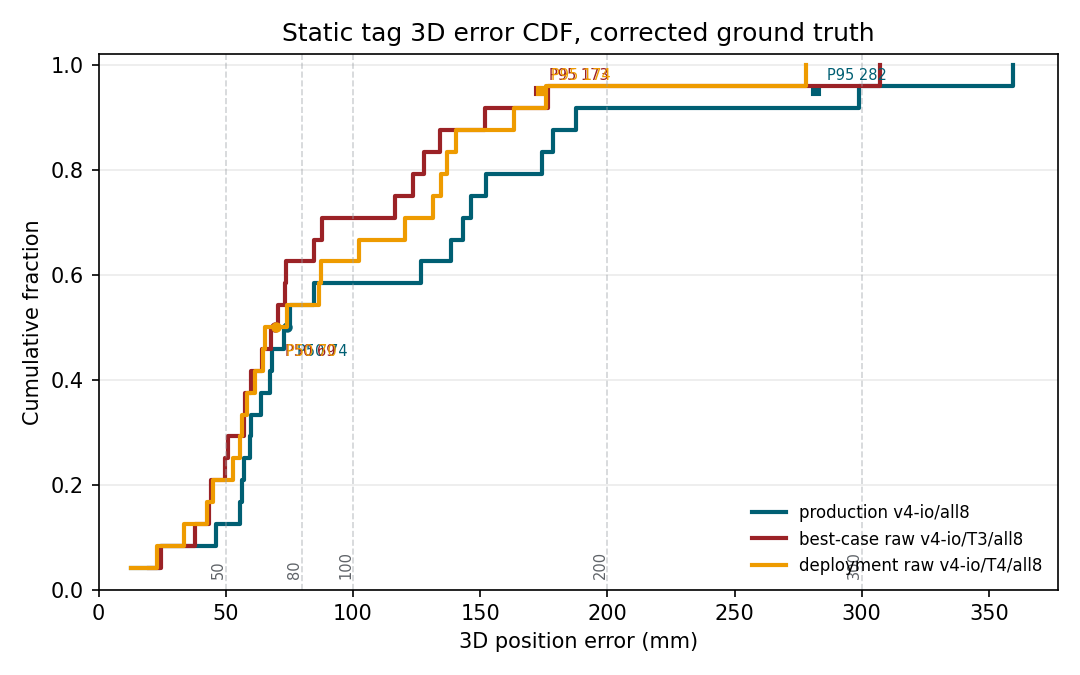
\includegraphics[width=\linewidth]{tag_error_cdf.png}
\caption{Original FULL static error CDF。}
\end{subfigure}
\hfill
\begin{subfigure}{0.49\textwidth}
\centering
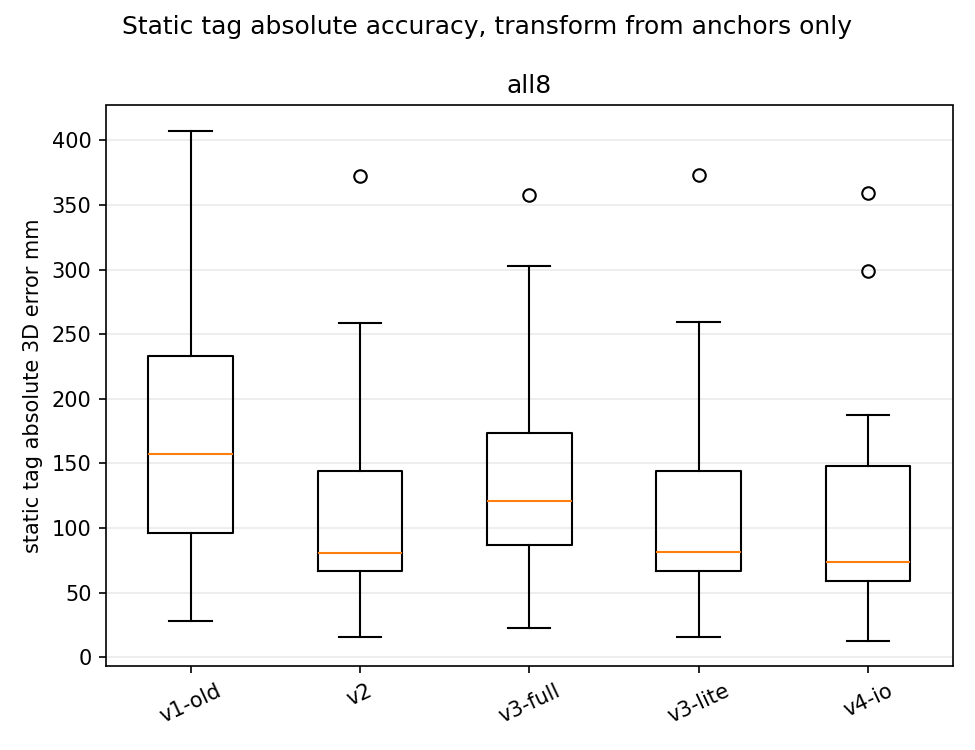
\includegraphics[width=\linewidth]{tag_error_by_position.png}
\caption{Static error by position。}
\end{subfigure}
\caption{静态误差具有明显的位置依赖和 tail behavior；单独一个 3D RMSE 不能完整表达误差结构。}
\end{figure}

\subsection{静态滤波与 Static-Lock 解释}

\begin{figure}[H]
\centering
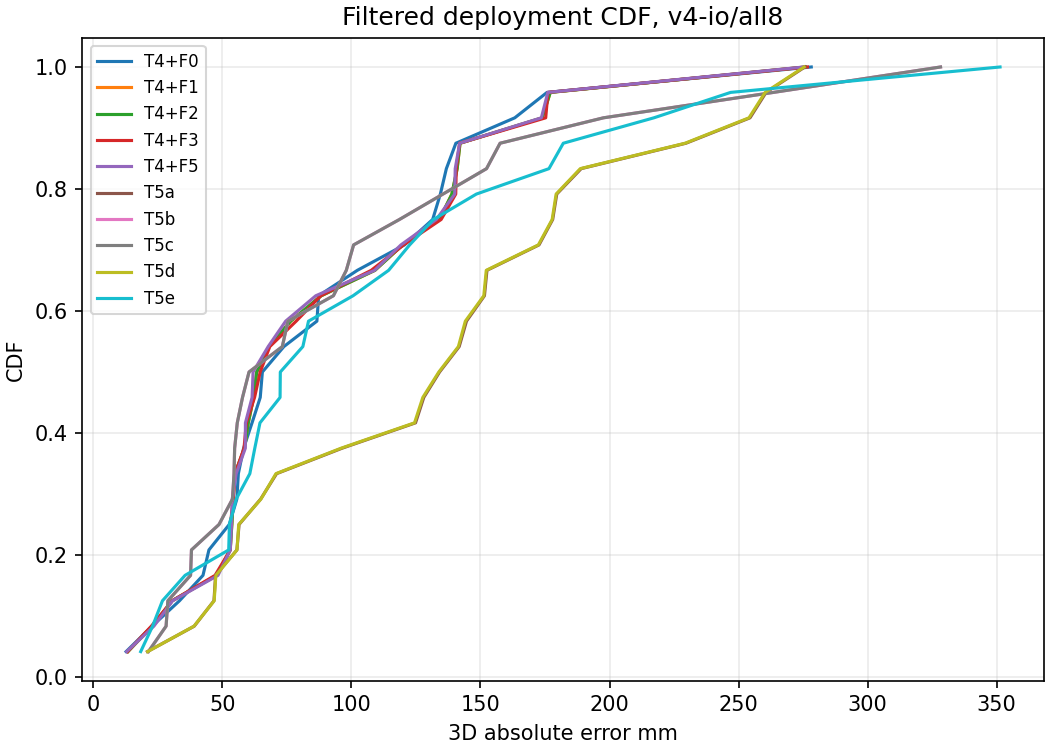
\includegraphics[width=0.8\textwidth]{filtered_static_cdf_v4io_all8.png}
\caption{静态 post-solve filtering。滤波可以降低用户看到的抖动，但不能消除系统性 layout/delay/ranging bias。}
\end{figure}

\begin{table}[H]
\centering
\tight
\caption{静态 stationary filter 结果。这些是 deployment/static-lock diagnostics，不是 raw calibration accuracy。}
\begin{tabular}{lrrrr}
\toprule
Solver & Median & P95 & RMSE & Repeatability SD median \\
\midrule
T4+F0 baseline & 69.7 & 173.9 & 108.9 & 67.4 \\
T4+F5 offline smoother & 64.9 & 175.7 & 109.5 & 18.7 \\
T4+F4 fixed-lag smoother & 65.9 & 176.1 & 109.6 & 21.4 \\
T3+F5 offline smoother & 65.2 & 169.9 & 105.4 & 21.0 \\
\bottomrule
\end{tabular}
\end{table}

如果应用知道 tag 是静止的，static-lock filtering 很有价值：它把 per-position 3D spread median
从 67.4 mm 降到 18.7 mm。但 P95 和 RMSE 与未滤波结果接近，因为 smoothing 不能去掉系统性 bias。

\section{动态 ROTO Absolute Trajectory Results}

\begin{figure}[H]
\centering
\begin{subfigure}{0.49\textwidth}
\centering
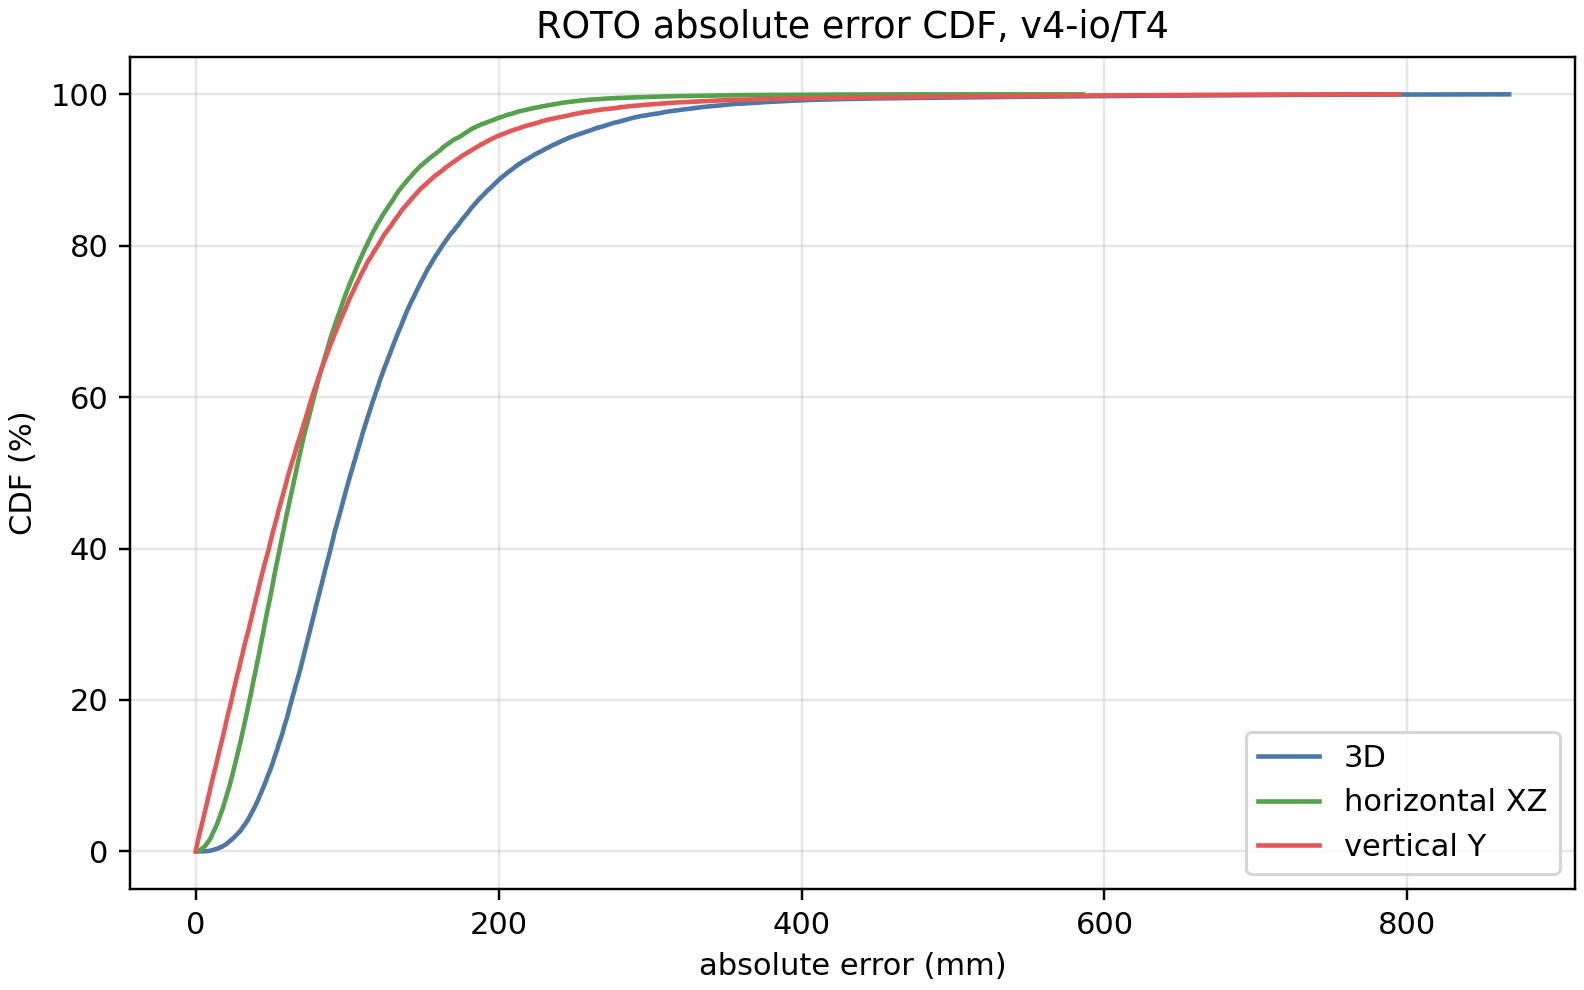
\includegraphics[width=\linewidth]{roto_abs_cdf_v4io_T4.png}
\caption{ROTO absolute error CDF。}
\end{subfigure}
\hfill
\begin{subfigure}{0.49\textwidth}
\centering
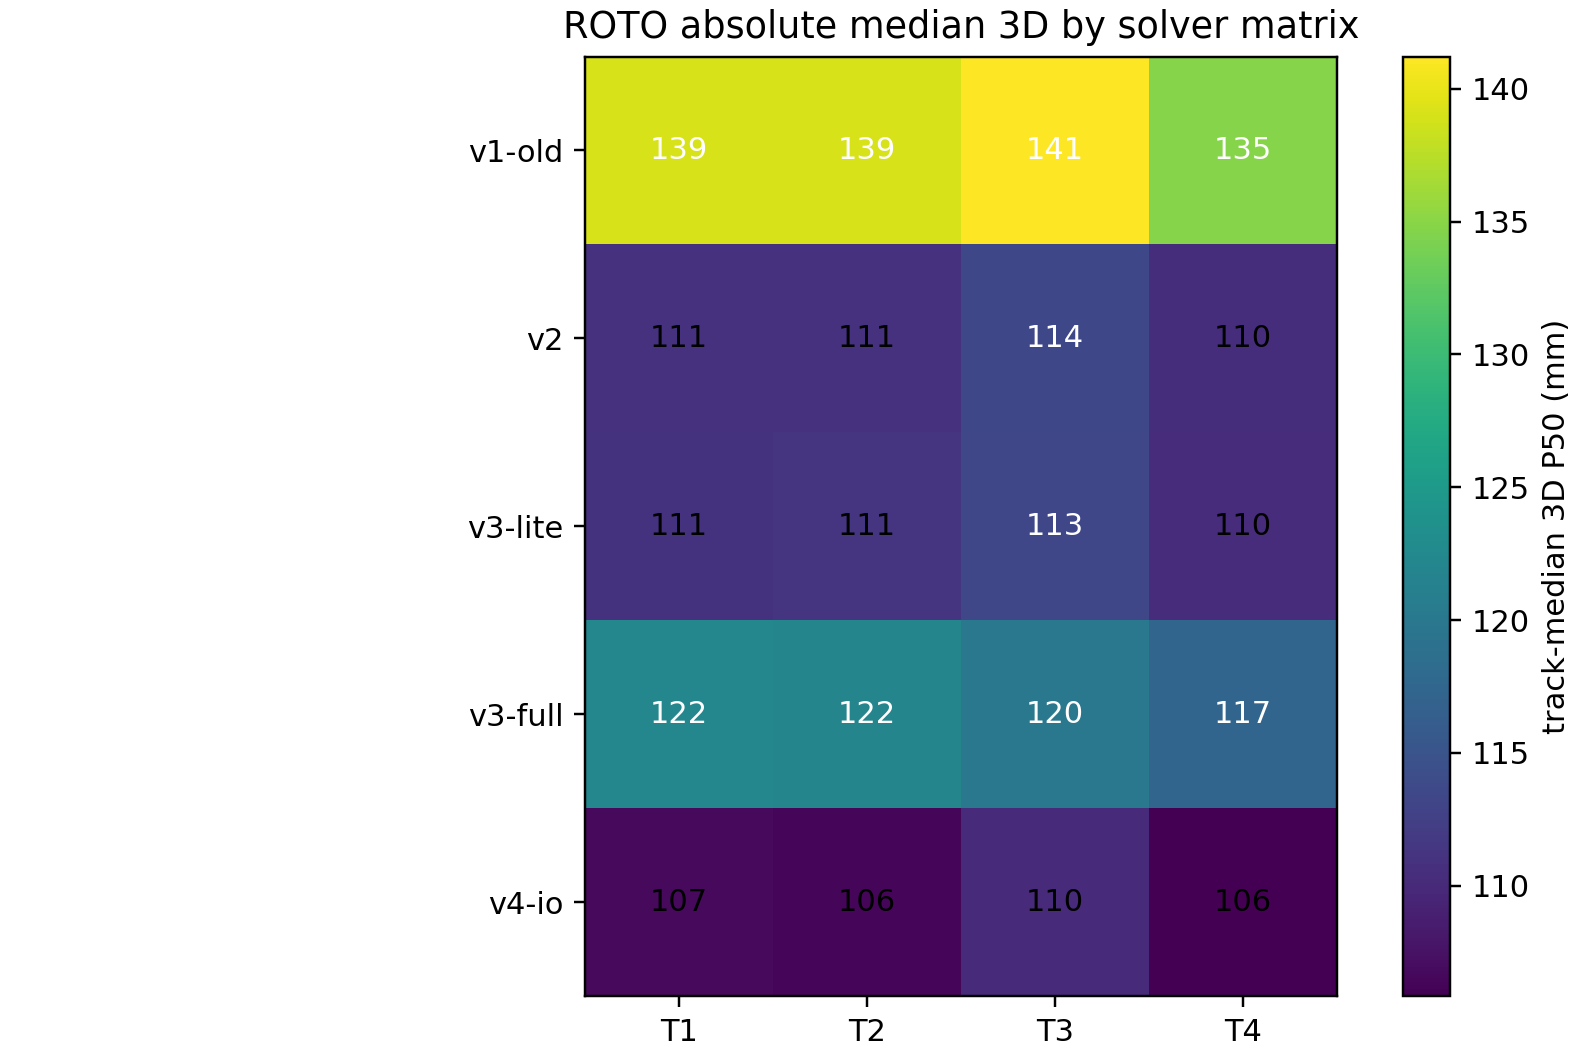
\includegraphics[width=\linewidth]{roto_solver_matrix_median3d.png}
\caption{ROTO solver matrix median 3D error。}
\end{subfigure}
\caption{动态 ROTO 在同一 T4 solver line 上仍接近 10 cm median。}
\end{figure}

\begin{table}[H]
\centering
\tight
\caption{ROTO absolute trajectory accuracy。P50/P95 为 track-median summary；RMSE 为 sample-pooled ATE RMSE。}
\begin{tabularx}{\textwidth}{lXrrr}
\toprule
Case & Layout/delay treatment & Track P50 & Track P95 & Sample RMSE \\
\midrule
FULL original \case{v4-io/T4} & self-cal layout + solver residual corrections & 105.8 & 231.8 & 141.3 \\
Vicon anchors + delaycal & known anchors + re-estimated delay & 105.6 & 200.4 & 125.4 \\
Sim(3) scale + delaycal & global scale removed + re-estimated delay & 110.5 & 200.7 & 127.8 \\
One-baseline E-H + delaycal & one-baseline scale + re-estimated delay & 106.2 & 200.4 & 126.7 \\
Best ROTO median row & one-baseline B-C with solver delay & 100.1 & 220.5 & -- \\
\bottomrule
\end{tabularx}
\end{table}

动态结果最重要的含义是：ROTO median 不会因为 layout 换成 Vicon anchors 并重新估计 delay 而崩到静态那样。
静态在 known-anchor delaycal 下可以从 108.9 mm RMSE 降到 77.7 mm RMSE；但 ROTO 仍约 105 mm median。
因此动态 ROTO 包含 motion、rotating-wand ranging behavior、antenna/marker geometry、trajectory residual
等因素，不只是静态 infrastructure calibration 的问题。

\begin{figure}[H]
\centering
\begin{subfigure}{0.49\textwidth}
\centering
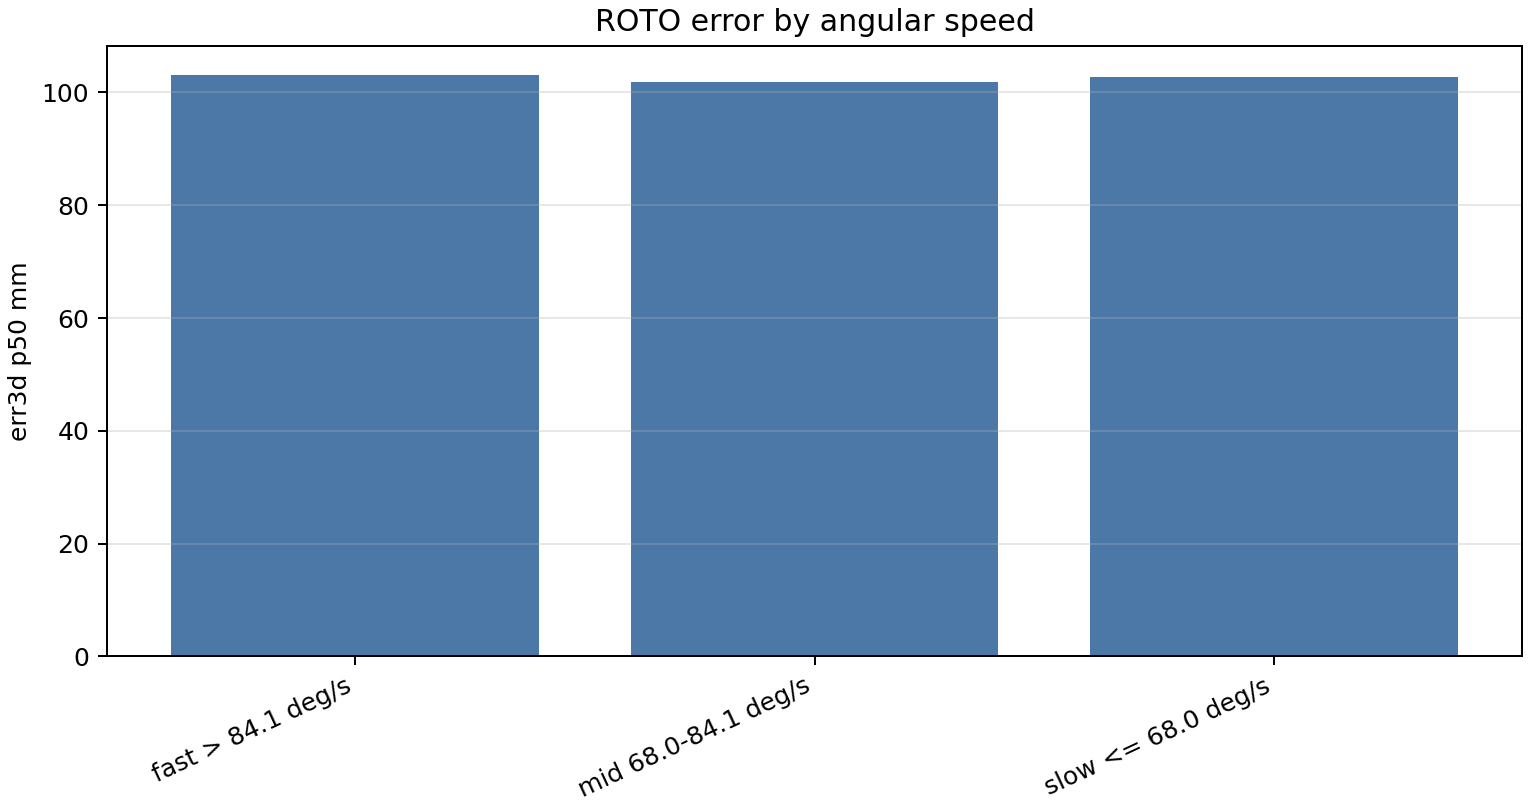
\includegraphics[width=\linewidth]{roto_error_by_angular_speed.png}
\caption{ROTO error by angular speed。}
\end{subfigure}
\hfill
\begin{subfigure}{0.49\textwidth}
\centering
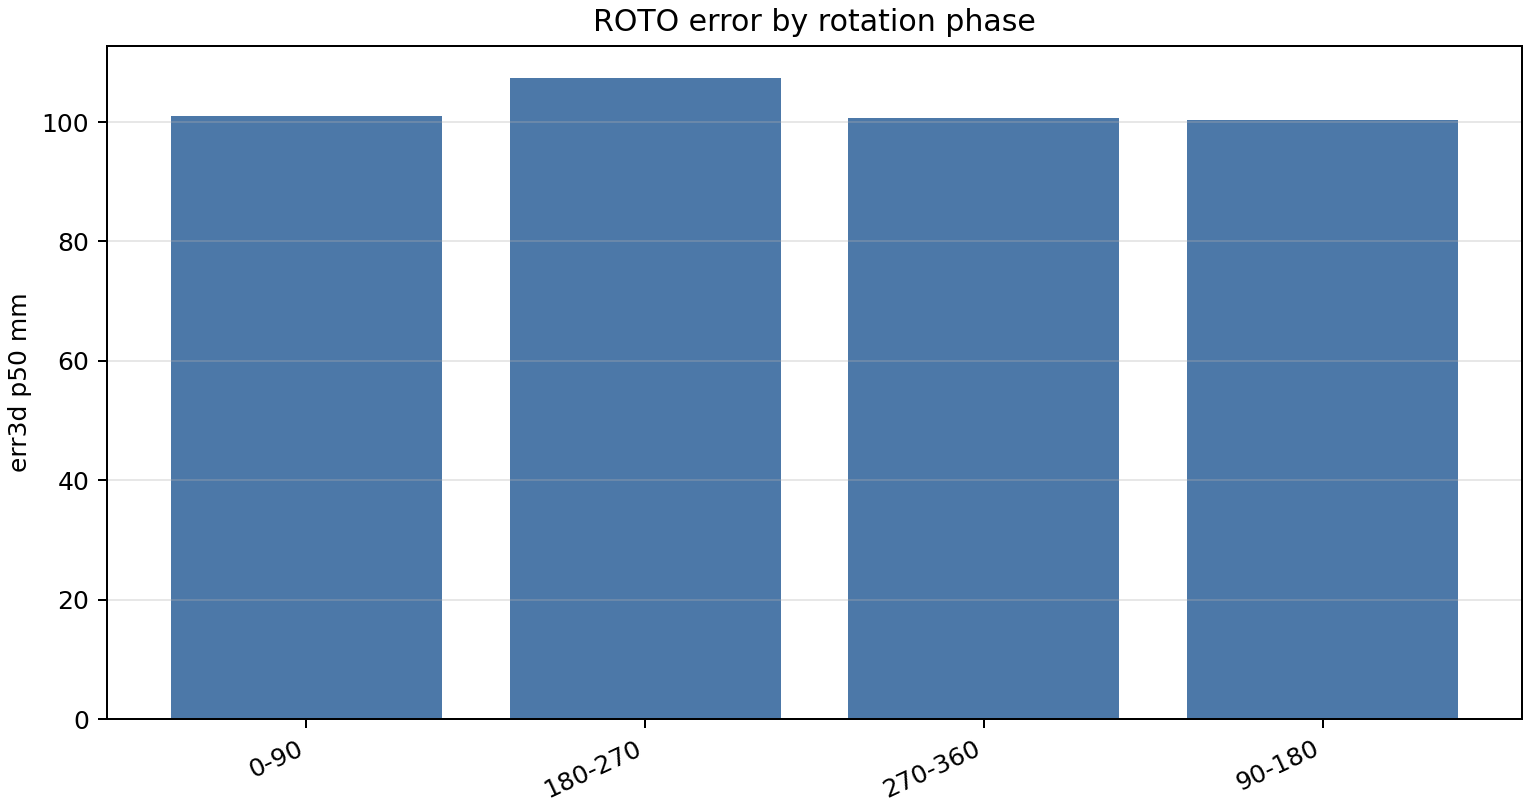
\includegraphics[width=\linewidth]{roto_error_by_phase.png}
\caption{ROTO error by phase。}
\end{subfigure}
\caption{Speed 与 phase 对 median 的影响有限，不能解释全部动态残差。}
\end{figure}

\subsection{Time Offset 与 Clock-Skew 证伪}

Reviewer audit 对每个 capture 重新拟合一个 constant time offset，然后又测试 affine time skew model：
\[
t_{\mathrm{query}} = t_{\mathrm{UWB}} + \beta + \alpha (t_{\mathrm{UWB}} - t_{\mathrm{ref}}).
\]
对于 original FULL \case{v4-io/T4}，sample-pooled P50 为：
当前 beta 102.63 mm、constant-offset refit 后 102.69 mm、skew refit 后 102.58 mm。
skew 只带来 0.11 mm pooled P50 的边际收益。拟合出的 median skew 为 -112 ppm，IQR 为 228 ppm，
verdict 为 \case{SKEW\_EXCLUDED}。在实际 ROTO 速度下，0.8 ms protocol window 只对应
0.51 mm median、0.72 mm P95 displacement。

\subsection{Single-Shot Static 与 ROTO}

静态数据也按 per-frame single-shot 方式 replay。对于 self-cal \case{v4-io/T4}，
static single-shot P50 为 89.6 mm，ROTO single-shot P50 为 102.6 mm，二者的 pooled 3D P50
动态 excess 约 13.1 mm。也就是说，静态 dwell averaging 的消失解释了一部分 static-vs-dynamic gap，
但 GDOP-conditioned bins 和 component-level 对比仍显示有限但真实的 dynamic term。Vicon-delaycal control
下 dynamic excess 更大，约 24.9 mm P50，这进一步支持动态 ROTO 不是单纯 layout-calibration artifact。

\subsection{旧 ROTO Self-Consistency 与新 OptiTrack Center Error}

旧的 no-groundtruth ROTO self-consistency metrics 仍有价值，但不能与 absolute trajectory error 混淆。
Original FULL \case{v4-io/T4}：
\begin{itemize}
    \item legacy radius-difference RMS 为 25.9 mm；
    \item turn-center repeatability median 为 13.7 mm；
    \item inner/outer center-separation median 为 37.6 mm；
    \item OptiTrack/Vicon turn-center absolute 3D RMS 为 72.1 mm。
\end{itemize}
该 absolute center RMS 在四条主路径上均约为 7--8 cm：original FULL 72.1 mm，
Vicon anchors + delaycal 72.7 mm，full similarity scale + delaycal 76.7 mm，
one-baseline E-H + delaycal 77.1 mm。

\section{ROTO Filtering 与 Pseudo-IMU Oracle}

\begin{table}[H]
\centering
\tight
\caption{Post-solve ROTO filtering。滤波作用在 solved positions 上，不重解 raw ranges。}
\begin{tabular}{lrrrr}
\toprule
Case & Track P50 & Track P95 & Sample RMSE & Center RMS \\
\midrule
FULL F0 baseline & 105.8 & 231.8 & 141.3 & 72.1 \\
FULL F4 fixed lag & 86.3 & 158.2 & 103.1 & 69.1 \\
FULL F5 offline RTS & 83.3 & 148.6 & 98.9 & 68.3 \\
Vicon F0 baseline & 105.6 & 200.4 & 125.4 & 72.7 \\
Vicon F4 fixed lag & 84.0 & 145.4 & 95.1 & 70.5 \\
Vicon F5 offline RTS & 82.7 & 139.1 & 91.2 & 70.0 \\
\bottomrule
\end{tabular}
\end{table}

Fixed-lag 与 offline smoothing 可以显著降低 dynamic scatter，但这是 trajectory-output/latency tradeoff，
不是 calibration improvement。Calibration-level claim 应保留 unfiltered ROTO；F4/F5 应作为
deployment-filter ablation 或 offline upper-bound diagnostic。

\begin{table}[H]
\centering
\tight
\caption{Pseudo-IMU oracle replay。Motion prior 来自 OptiTrack marker motion，并已 lever-arm 到 UWB antenna point。}
\begin{tabular}{lrrrrr}
\toprule
Case & Fusion & Track P50 & Track P95 & Sample RMSE & dR RMS \\
\midrule
FULL original & PI0 baseline & 105.8 & 231.8 & 141.3 & 25.9 \\
FULL original & PI1 causal oracle & 66.1 & 97.5 & 71.6 & 12.3 \\
FULL original & PI4 offline oracle & 58.7 & 81.5 & 61.8 & 5.3 \\
Vicon delaycal & PI0 baseline & 105.6 & 200.4 & 125.4 & 18.0 \\
Vicon delaycal & PI1 causal oracle & 64.0 & 100.2 & 69.8 & 11.7 \\
Vicon delaycal & PI4 offline oracle & 59.9 & 82.0 & 63.1 & 4.3 \\
\bottomrule
\end{tabular}
\end{table}

Body-fit antenna prior residual 只有 0.6 mm P50-of-P50 / 1.5 mm P50-of-P95，
说明 pseudo-IMU 不是错误地把 marker body centroid 当成 antenna point。但它仍然是 oracle：
motion prior 来自 OptiTrack，而不是真实 IMU。论文中应表述为：一个正确 lever-armed 的 inertial
relative-motion channel 值得实现并验证，而不是当前系统已经具备 deployable UWB+IMU result。

\section{鲁棒性与 Reporting Checklist}

\begin{table}[H]
\centering
\tight
\caption{Numerical precision 与 dropout stress。Bootstrap 结果不是 independent deployment repeatability。}
\begin{tabularx}{\textwidth}{lXrrrr}
\toprule
Case & Diagnostic & Coord SD & Delay rel-A SD & Static P50/P95 & Note \\
\midrule
Original self-cal & raw-pair median bootstrap & 1.02 & 0.56 & 76.3/180.9 & within-campaign sampling SE \\
Vicon truth + delaycal & residual-delay bootstrap & 0.00 & 0.45 & 65.0/126.7 & coordinate fixed by control \\
Sim(3) scale + delaycal & raw-pair median bootstrap & 0.97 & 0.53 & 69.3/134.8 & within-campaign sampling SE \\
One-baseline E-H & raw-pair median bootstrap & 1.20 & 0.54 & 60.6/127.9 & within-campaign sampling SE \\
\bottomrule
\end{tabularx}
\end{table}

Raw-pair bootstrap 不能写成 deployment repeatability。它与 analytical median sampling standard error
一致，因此反映的是同一 campaign 内 large-\(n\) numerical precision。仍然缺少的真正证据包括：
independent repeated AutoPos deployments、true repeated-run residual-delay SD、同数据集 PANS/manual baseline、
显式 CIR/NLOS label，以及 raw dynamic ROTO range re-solve under physical packet loss。

Static dropout stress 是从 raw static frames 重新解算的。Original self-cal 在 random per-frame four-anchor
stress 下，从 76.3/180.9 mm 变为 87.7/292.4 mm position P50/P95，并且 sample-level spread 明显变差。
Fixed-random four-anchor subsets 与 best-GDOP four-anchor subsets 将 non-convergence 显式报告出来；
它们的 P50/P95 是 conditional on convergence。ROTO packet stress 目前是 solved-sample thinning，
不是 raw range re-solve：ATE 在 thinning 下相对稳定，但随着 effective update rate 从约 10 Hz 降到约 1 Hz，
RPE 明显变差。

\section{Per-Tag 与 Per-Anchor Residual Structure}

WHY \#9 的 two-way median-polish decomposition 将 common-mode、tag main effect、anchor main effect
和 tag-anchor interaction 拆开。Pairwise tag residual range offsets 在 self-cal 与 Vicon-delaycal
两个场景之间非常稳定：
\begin{itemize}
    \item BS2DCE minus BSF66F：self-cal 31.0 mm，Vicon-delaycal 34.6 mm；
    \item BSDC91 minus BSF66F：self-cal -12.7 mm，Vicon-delaycal -11.7 mm；
    \item BS2DCE minus BSDC91：self-cal 43.7 mm，Vicon-delaycal 46.3 mm。
\end{itemize}
这些 tag difference 最大跨场景变化只有 3.6 mm，median interaction term 只有 0.9 mm 和 2.4 mm。
因此它们可以作为 deployable per-tag range-offset trim targets。但措辞上要克制：这是 per-tag range offset，
它把 device antenna delay、固定安装偏置、稳定 power/ranging bias 合并成一个 scalar correction；
不能直接声称已经单独测出了 antenna delay。

Anchor side 则不同。仅依靠 tag-to-anchor ranges，absolute per-anchor 和 per-tag delay 不可分，
因为存在 global delay/scale gauge coupling。Self-cal anchor residual structure 会吸收 layout radial error，
所以 self-cal \case{d\_anchor} 应写作 layout-level residual correction，而不是 physical anchor antenna-delay measurement。

\section{建议写入论文的 Claims}

\begin{enumerate}
    \item 部署静态 headline 使用 unfiltered production mean-aggregated \case{v4-io/T4}：
    \textbf{72.7 mm median / 171.5 mm P95 / 109.8 mm RMSE}。
    \item \case{69.7/173.9 mm} 只作为同一 solver line 的 median-estimator ablation，不写成 deployed production output。
    \item FULL-US 应写成 BioSpur UWB+US30 的 deployment-gauge variant。不要把它写成相对 FULL
    在 legacy anchor-locked metric 下的显著 accuracy improvement；它的贡献是固定具有物理意义的
    vertical gauge。可引用 height-preserving \case{v4-io} 静态诊断：
    \textbf{72.5/284.8 mm}，RMSE \textbf{139.1 mm}。
    \item Known-anchor + re-estimated-delay control 是 diagnostic control，不是普通 lower bound：
    它是 64.1/128.4 mm、77.7 mm RMSE 的最佳静态 control，但需要 OptiTrack anchors 与重新估计 residual delay。
    \item Delay-layout coupling 是核心结果：311/252/77 mm triangle 与 \(R^2=0.998\)、slope \(-0.982\)
    radial-absorption mechanism 是同一 non-separability 的 outcome view 与 mechanism view。
    \item ROTO 应保守表述：unfiltered dynamic absolute trajectory error 约为 10 cm median，
    P95 约为 20--23 cm，具体取决于 control row。
    \item F4/F5 filtering 与 PI1/PI4 pseudo-IMU 只能作为 deployment-filter diagnostic 或 oracle upper bound，
    不能写成 calibration accuracy。
    \item 不要只报告一个 3D RMSE。应拆开 repeatability、absolute error、scale bias、shape distortion、
    delay-layout coupling、downstream tag error 与 tail behavior。
\end{enumerate}

\section{局限性与下一步实验}

当前数据集已经较完整地覆盖了 corrected OptiTrack-isolated FULL analysis，但还缺少几类独立证据：
\begin{itemize}
    \item independent repeated AutoPos deployments 或 layout splits；
    \item true repeated-run residual-delay standard deviation；
    \item 同一数据集下 practical PANS/manual baseline；
    \item 与每条 link 对齐的 explicit CIR/NLOS labels；
    \item raw dynamic ROTO range re-solve under physical packet loss；
    \item 带 IMU-to-UWB-antenna extrinsic calibration 的真实 IMU 数据。
\end{itemize}

最值得继续做的是真实 UWB+IMU fusion。Pseudo-IMU oracle 已经说明：正确 lever-armed 的 relative-motion prior
有足够 leverage，可以把 ROTO 从 105.8/231.8 mm 降到 strong causal oracle 下的 66.1/97.5 mm。
部署版本应使用真实 inertial measurements、antenna-frame extrinsic calibration，以及 raw-range EKF/UKF，
而不是只对 solved positions 做 smoothing。

\section{源文件与产物}

本文基于以下已生成产物：
\begin{itemize}
    \item \case{FULL\_4way\_comparison/reports/FULL\_4WAY\_BIG\_COMPARISON.md}
    \item \case{FULL\_4way\_comparison/reviewer\_audit/reports/MEASUREMENT\_REVIEWER\_AUDIT.md}
    \item \case{FULL\_4way\_comparison/reporting\_checklist/reports/REPORTING\_CHECKLIST\_AUDIT.md}
    \item \case{FULL\_4way\_comparison/resilience\_gap\_audit/reports/RESILIENCE\_GAP\_AUDIT.md}
    \item \case{FULL\_4way\_comparison\_US/reports/FULL\_4WAY\_BIG\_COMPARISON.md}
    \item \case{FULL\_NO\_US\_VS\_US/reports/FULL\_NO\_US\_VS\_US\_COMPARISON.md}
    \item \case{FULL\_4way\_comparison/tables/full\_4way\_headline\_comparison.csv}
    \item \case{FULL\_4way\_comparison/reporting\_checklist/tables/*.csv}
    \item \case{FULL\_4way\_comparison/reviewer\_audit/tables/why*.csv}
\end{itemize}

\end{document}
